\documentclass[border=10pt]{standalone}

\usepackage{tikz}
\usepackage{tikzsymbols}
\usetikzlibrary{calc,patterns,shapes.geometric}

\def\centerarc[#1](#2)(#3:#4:#5){\draw[#1] ($(#2)+({#5*cos(#3)},{#5*sin(#3)})$) arc (#3:#4:#5);}

\begin{document}
	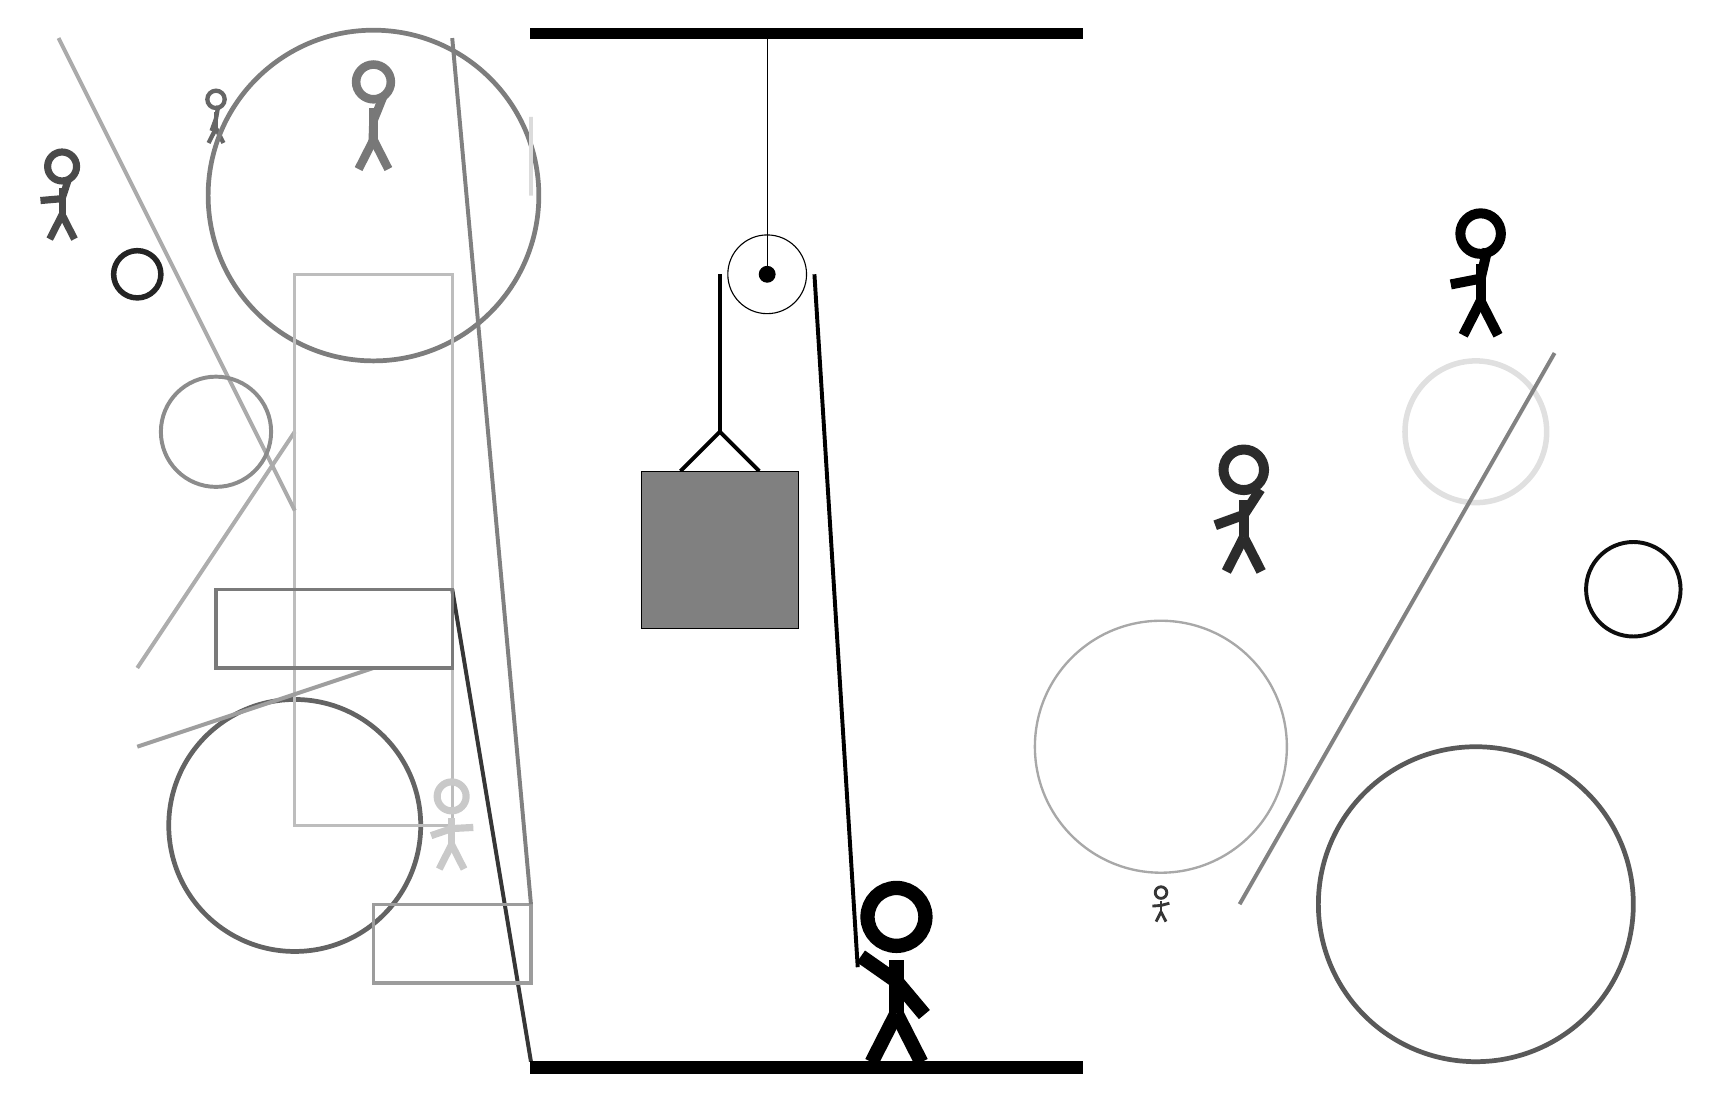
\begin{tikzpicture}
		%%%%% START %%%%%
		
		\draw[fill=black] (-2, 10) rectangle (5, 10.125);
		
		\draw (1, 7) circle (0.5);
		\draw[fill=black] (1, 7) circle (0.1);
		\draw (1, 10) -- (1, 7);
		
		\draw [line width=0.7mm, color=black!12](10, 5) circle (0.9);
		
		\draw[line width=0.5mm, color=black!79](-2, -3) -- (-3, 3);
		\node[line width=0.4mm, color=black!60] at (-6, 9) {\Strichmaxerl[3][70][80]};
		\draw [line width=0.6mm, color=black!51](-4, 8) circle (2.1);
		
		\node[line width=0.5mm, color=black!83] at (7, 4) {\Strichmaxerl[7][20][57]};
		
		\draw[line width=0.5mm, color=black!32](-7, 2) -- (-5, 5);
		\node[line width=0.3mm, color=black!100] at (10, 7) {\Strichmaxerl[7][11][77]};
		\draw [line width=0.6mm, color=black!61](-5, 0) circle (1.6);
		\draw [line width=0.5mm, color=black!95](12, 3) circle (0.6);
		\draw[line width=0.4mm, color=black!39] (-4, -2) rectangle (-2, -1);
		
		\draw [line width=0.7mm, color=black!86](-7, 7) circle (0.3);
		\draw [line width=0.3mm, color=black!34](6, 1) circle (1.6);
		\draw[line width=0.5mm, color=black!49](7, -1) -- (11, 6);
		
		\draw [line width=0.6mm, color=black!65](10, -1) circle (2.0);
		\draw[line width=0.4mm, color=black!14] (-2, 8) rectangle (-2, 9);
		\node[line width=0.3mm, color=black!53] at (-4, 9) {\Strichmaxerl[6][88][68]};
		\draw[line width=0.5mm, color=black!50](-2, -1) -- (-3, 10);
		\draw[line width=0.4mm, color=black!26] (-3, 0) rectangle (-5, 7);
		\draw[line width=0.5mm, color=black!33](-5, 4) -- (-8, 10);
		
		\node[line width=0.2mm, color=black!71] at (-8, 8) {\Strichmaxerl[5][5][72]};
		\draw [line width=0.5mm, color=black!45](-6, 5) circle (0.7);
		\draw[line width=0.5mm, color=black!38](-4, 2) -- (-7, 1);
		
		\node[line width=0.6mm, color=black!79] at (6, -1) {\Strichmaxerl[2][4][15]};
		\draw[line width=0.4mm, color=black!52] (-3, 2) rectangle (-6, 3);
		\node[line width=0.3mm, color=black!21] at (-3, 0) {\Strichmaxerl[5][19][3]};
		
		\draw[line width=0.5mm] (-0.1, 4.5) -- (0.4, 5.0) -- (0.9, 4.5);
		\draw[fill=black!50] (-0.6, 4.5) rectangle (1.4, 2.5);
		
		\draw[line width=0.5mm] (0.4, 7) -- (0.4, 5.0);
		\centerarc[line width=0.5mm](1, 7)(0:180:0.6);
		\draw[line width=0.5mm](1.6, 7) -- (2.15, -1.8);
		
		\node at (2.6, -1.9) {\Strichmaxerl[10][-35][-50]};
		
		\draw[fill=black] (-2, -3) rectangle (5, -3.15);
		
		%%%%% END %%%%%
	\end{tikzpicture}
\end{document}